\documentclass[12pt, a4paper]{article}
\usepackage[margin=0.5in]{geometry}

\usepackage{color}
\usepackage[dvipsnames]{xcolor}
\usepackage{hyperref}
\hypersetup{
    colorlinks=true,
    linkcolor=blue,
    urlcolor=blue,
    linktoc=all
}


\usepackage{amsmath}
\usepackage{mathtools}
\usepackage{amssymb}
\usepackage{cancel}
\usepackage{bm}
\usepackage{dsfont}
\usepackage{graphicx}
\usepackage{graphics}
\usepackage{xfrac}
\usepackage{array}
\setcounter{MaxMatrixCols}{40}

\usepackage{enumerate}
\usepackage{enumitem}
\usepackage{multirow}

%inclusions carried over from past class homework formats
\usepackage{units}
\usepackage{fullpage}
\usepackage{alltt}
\usepackage{mathrsfs}
\usepackage{xcolor}
\usepackage{soul}

\usepackage{pgfplots}

\DeclarePairedDelimiter{\abs}{\lvert}{\rvert}
\newcommand*{\fontCourier}{\fontfamily{pcr}\selectfont}
\newcommand*\mean[1]{\overline{#1}}
\newcommand\scalemath[2]{\scalebox{#1}{\mbox{\ensuremath{\displaystyle #2}}}}

\setcounter{tocdepth}{5}
\setcounter{secnumdepth}{5}

\usepackage{pdfpages}
\usepackage{Sweave}
\begin{document}
% 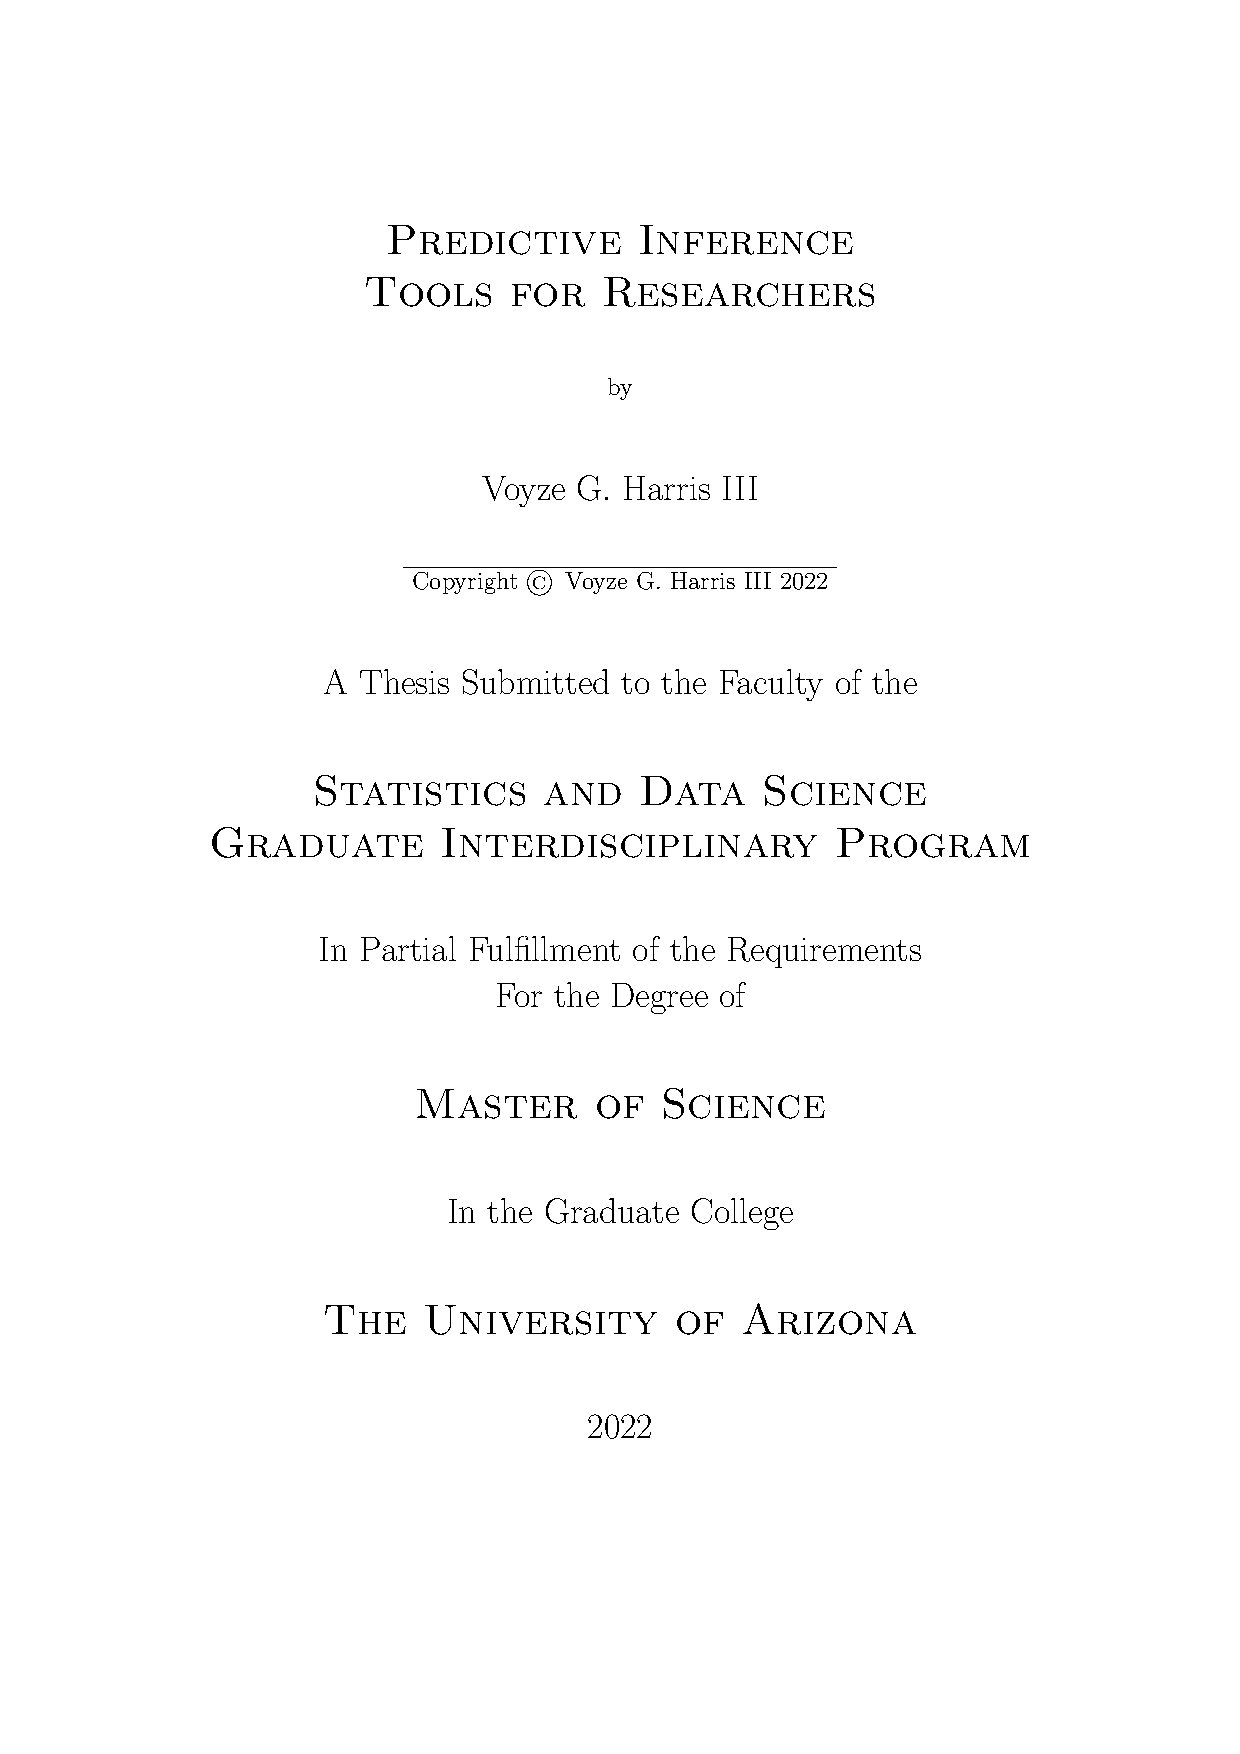
\includepdf{TitlePage_MastersThesis}
% 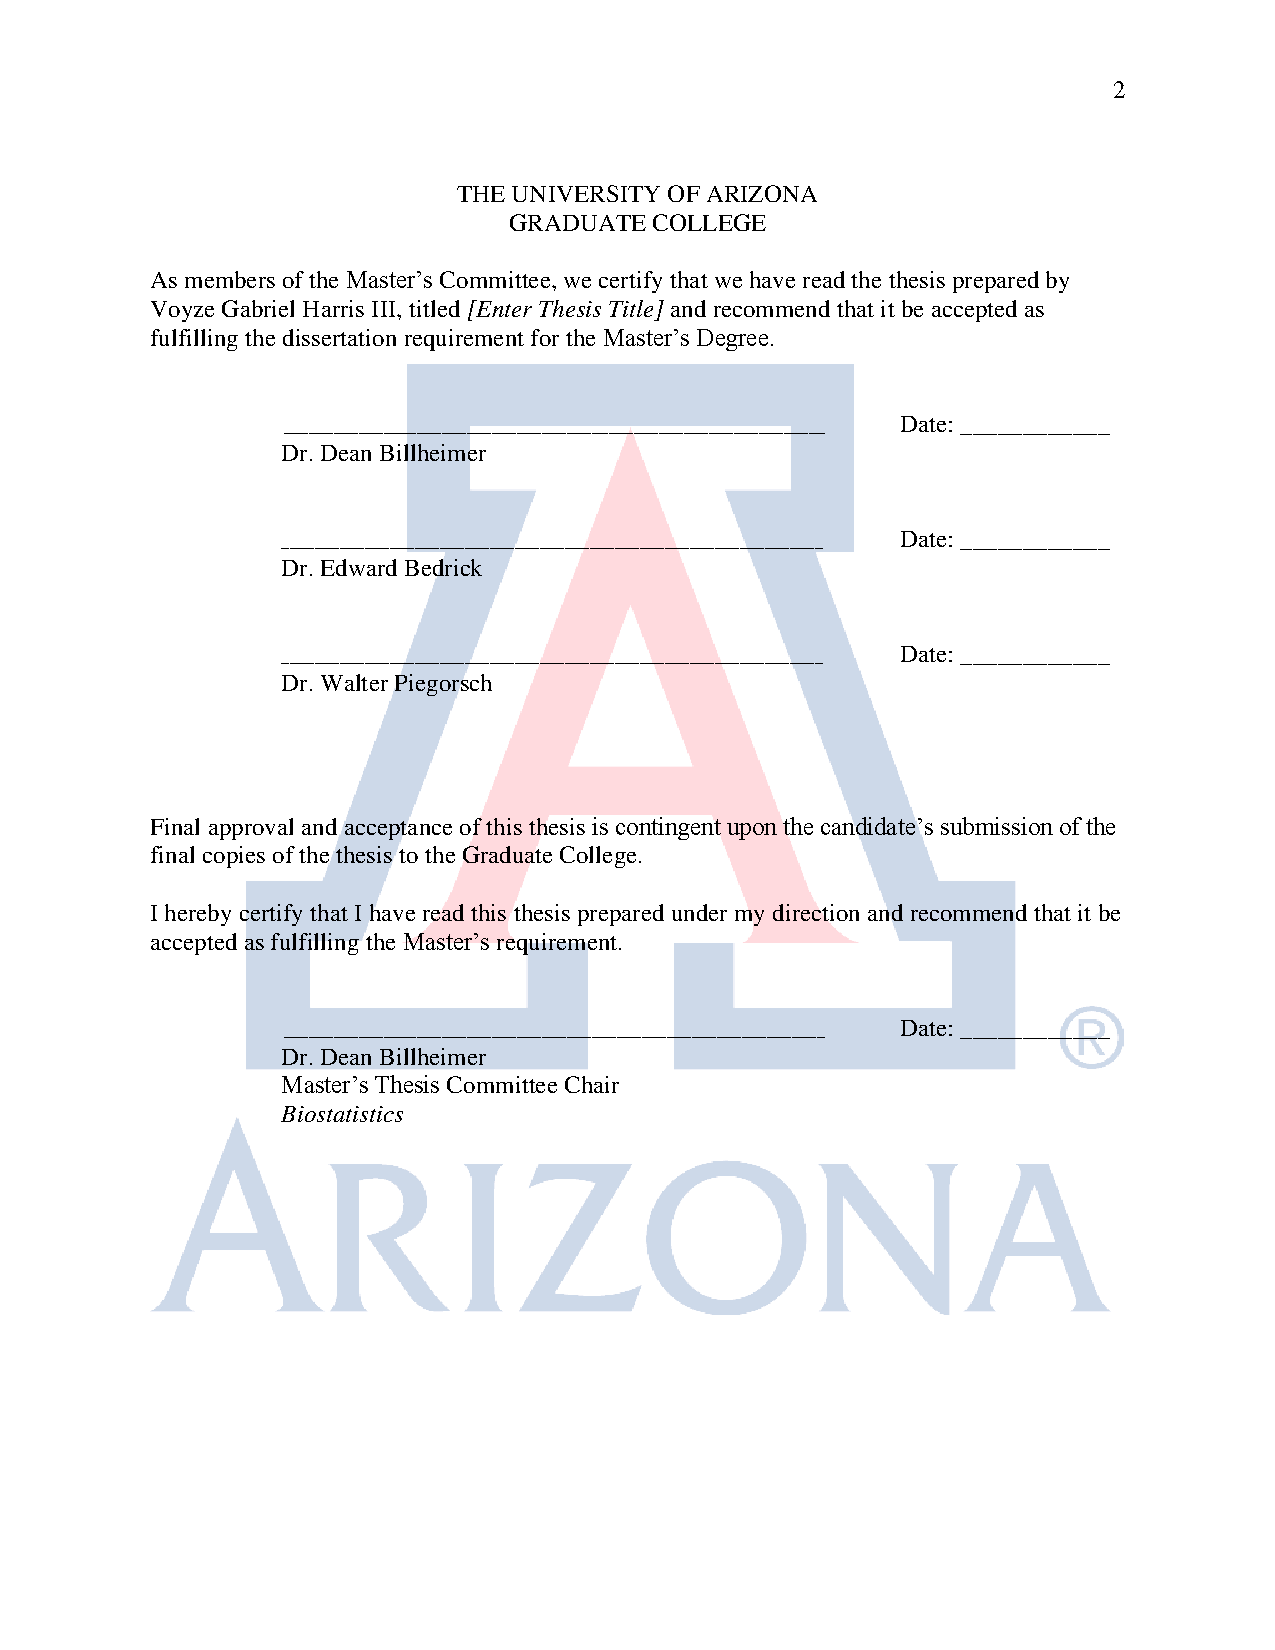
\includepdf{ThesisApprovalPage}
\Sconcordance{concordance:DeanArticleNotes.tex:DeanArticleNotes.Rnw:%
1 49 1 1 0 7 1 1 4 66 1}


% \tableofcontents
% \newpage



\title{Notes on ``Predictive Inference and Scientific Reproducibility" by Dean Billheimer}
\author{\Large Gabe Harris}
\maketitle

\textbf{Abstract}\\
\begin{itemize}
  \item hypothesis tests & parameter estimation for inference are ``noble, but misguided."
  \item "observables are fundamental"
  \item prediction of future events is the goal of statistical modeling
  \item obvious benefits (see list)
  \item avoidance of inference about parameters which are imaginary entities "that exist only as convenient indices of hypothetical distributions"
  \item shift focus from "finding differences among hypothetical parameters to predicting observable events based on our current scientific understanding."
\end


\end{document}
